\chapter*{\FontH{\Huge Löwenalarm}}
\addcontentsline{toc}{chapter}{Löwenalarm}
\lettrine[lines=3]{\color{DeepPink}M}{ama} und Papa schlafen noch. Mama wie üblich etwas lauter als Papa.  Sehr wohlig klingt das. Ich hatte mich zwar erst auch noch zu ihnen gelegt, aber das war diesmal doch zu langweilig, lieber gleich wach bleiben. 

Der aufregendste Ort bei mir zuhause ist die oberste Schublade im Schreibtisch von Mama. Eigentlich darf ich die gar nicht aufmachen, denn dort gibt es auch eine Schere und Reisszwecken und allerhand andere Dinge, die für mich gefährlich sein könnten. Behaupten jedenfalls Mama und Papa und die sagen, dass man mindestens sechs Jahre alt sein muss, um da aufmachen zu dürfen. Aber ich kann ja spielen, ich sei schon so alt. 

Tausend Dinge gibt es in dieser Schublade. Bei den meisten weiss ich gar nicht, wozu die gut sind. Zum Spielen sind sie jedenfalls prima geeignet. Eine Dose mit kleinen silbernen Dingern geht erst nicht auf, dann purzeln alle auf den Boden. Ein Lineal kommt zum Vorschein, das kenne ich schon. Eine 1A-Rutschbahn gibt das Lineal, wenn man es schräg hält. Nach und nach dürfen alle Schubladenbewohner die Rutsche einmal ausprobieren. Wer vor dem Ende abstürzt ist blöd. 

Ganz hinten in der Schublade entdecke ich einen Stift, den ich noch nie gesehen habe. Der ist ganz dick und bunt. Aha, wenn man hier drückt, kann man rot schreiben und wenn man hier drückt blau. Gelb und Schwarz gibt es auch und Rosa -- meine Lieblingsfarbe -- ist auch dabei.

Zum Stift fehlt noch Papier, das liegt im Arbeitszimmer. Da kann ich gleich noch auf dem Stuhl im Kreis drehen und spielen, dass ich Rennauto fahre. Aber zuerst Malen. 

Der erste Strich ist rosa. Die Farbe passt ja wohl nur zu Feen, also fange ich an, eine Fee zu malen. Erst eine grosse Fee, dann noch eine und dann noch drei kleine dazu. Eine Feenfamilie mit zwei Mamas. Aus dem Schlafzimmer höre ich \emph{meine} Mama immer noch schnarchen. Wie ein Löwe klingt das, also male ich auch noch einen Löwen. Der bekommt eine grosse Mähne aus Kringeln und einen aufgerissenen Mund. Der Löwe brüllt nämlich gerade. Und spitze Zähne hat der auch, die muss man ganz vorsichtig malen, die sind gefährlich!

Und jetzt noch einen Knochen für den Löwen zum Fressen, der soll blau werden, aber irgendwie will der Stift nicht mehr blau malen. Also ab ins Kinderzimmer einen blauen Stift suchen.

Als ich endlich einen gefunden habe und zurückkomme, da sind die Feen weg! Verschwunden! Nicht mehr da! Die Papierblätter liegen noch genau da wo ich sie gelassen habe, der Löwe ist auch noch da, aber die Feen sind weg.

Ich suche sie in der ganzen Wohnung. Nur gut, dass ich so oft mit Mama und Papa Verstecken-spielen übe. Ich kenne jetzt alle Verstecke bei uns zuhause. Papa ist immer hinter der Tür, da sind die Feen aber nicht. Auch nicht in Mamas Lieblingsversteck, gleich neben der Couch. Nein, unter dem Waschbecken, da wo ich mich immer verstecke, finde ich sie. Dort sitzen sie und haben sich ganz fest aneinander geklammert.

\enquote{Hilfe!}, rufen sie, \enquote{Ein riesiger Löwe war eben da, der hatte den Mund ganz weit offen und die Zähne hatte er geflätscht. Die waren so spitz wie die gefährlichste Schere der Welt. Der wollte uns bestimmt fressen!}

\afterpage{
\begin{figure}
    \vspace{3cm}
\centering
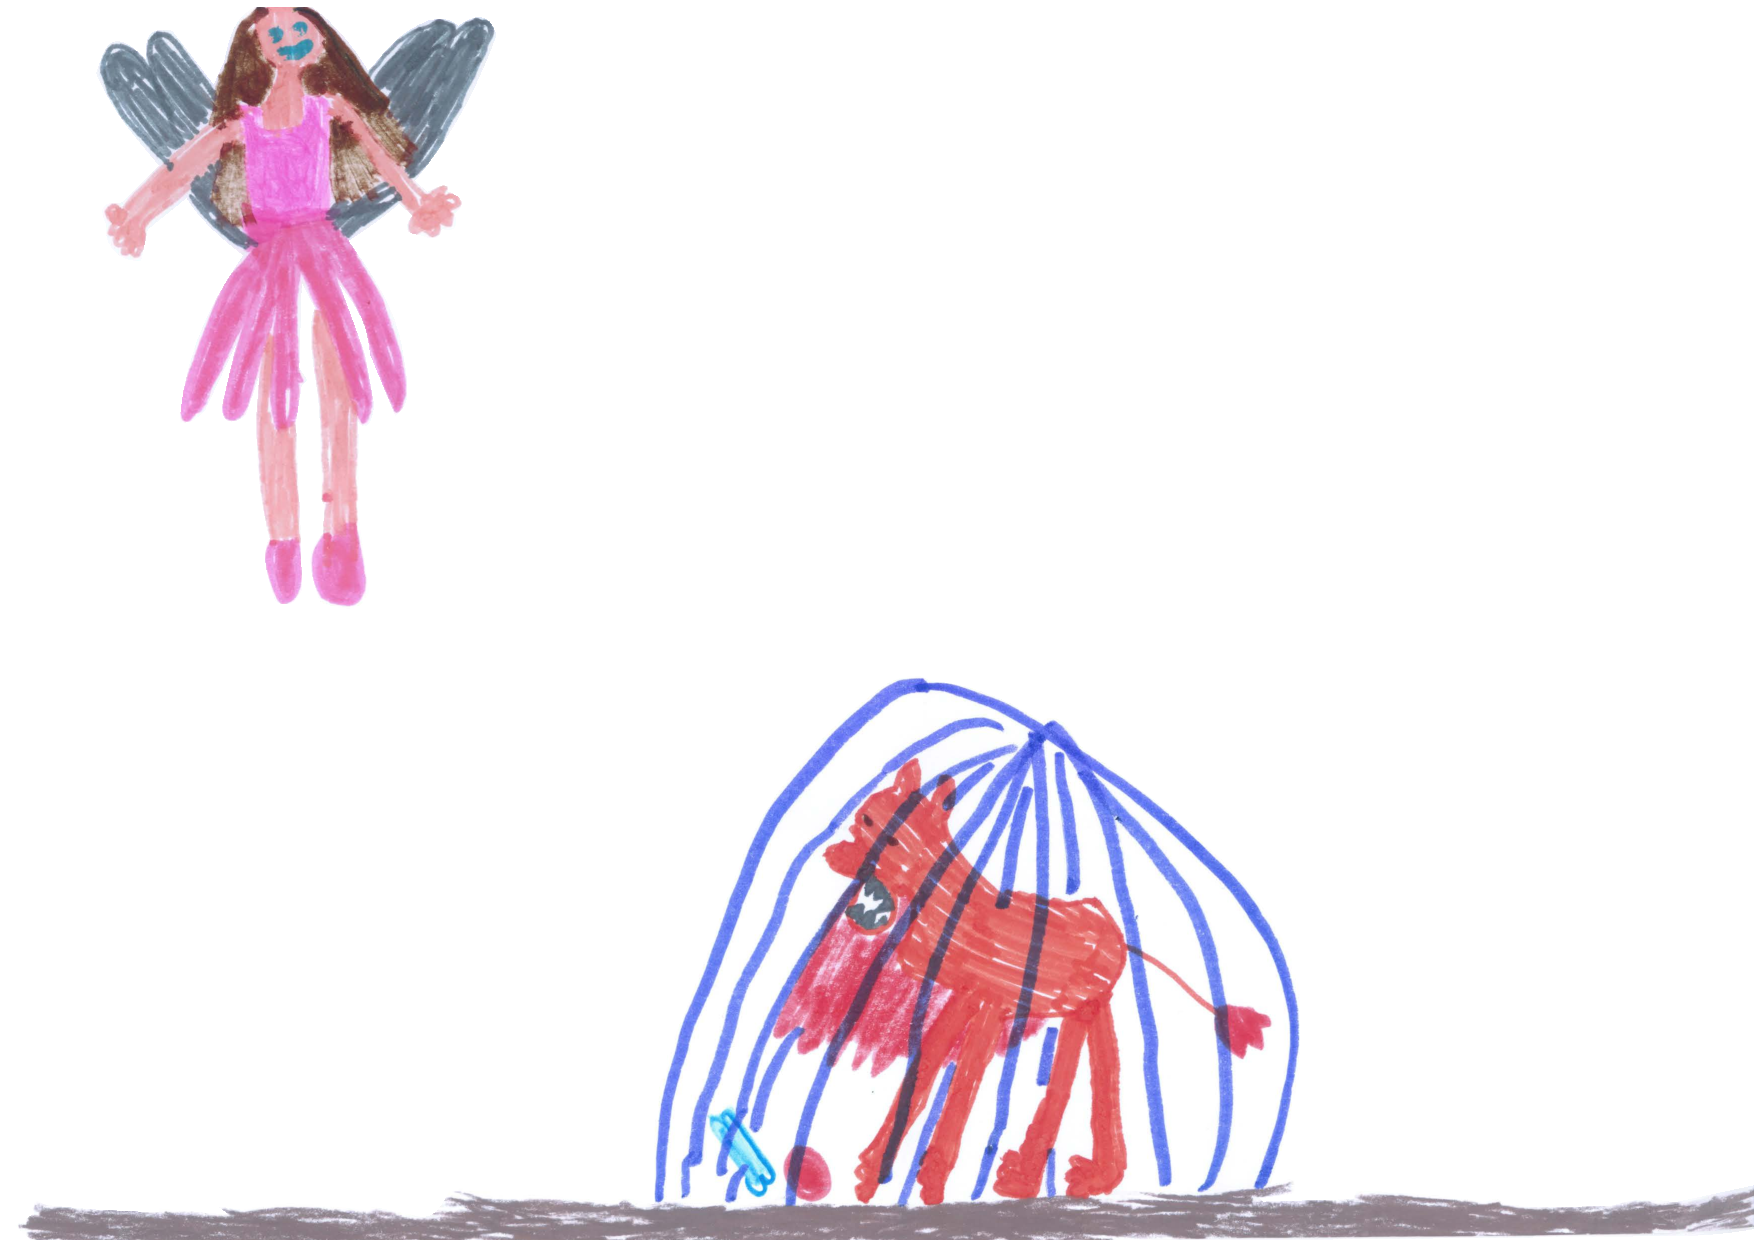
\includegraphics[width=\textwidth,height=.7\textheight]{bilder/loewenalarm.pdf}
\end{figure}
\clearpage
}



Oh je. Jetzt haben die Feen Angst vor dem Löwen bekommen. Das habe ich nicht gewollt, daran hatte ich nicht gedacht beim Malen.  Ich versuche die Feen zu beruhigen, aber es hilft nichts. Immer wieder rufen sie \enquote{Wir haben Angst!}, und
\begin{center}
 {\color{DeepPink}
\large
\itshape
\enquote{LÖ --- WEN --- A --- LARM}}
\end{center}

Dann habe ich eine gute Idee. Ich nehme den blauen Stift und male statt dem Knochen lieber noch einen Käfig um den Löwen. Dicke schwere Gitter und ein Schloss, so gross wie es nur Platz hat. Da kommt der nicht raus, der ist jetzt im Gefängnis einer ganz dicken Burg. Und ich male noch einen Apfel, um zu zeigen, dass das ein Löwe ist, der lieber Äpfel als Feen ist. Gerade will ich das Bild den Feen wieder zeigen, da sehe ich, dass alle Feen wieder zurück in das Bild gekommen sind. Erst eine und dann die anderen hinterher. Genau wie vorhin fliegen sie durch die Luft und verteilen Feenstaub. 

Da bin ich beruhigt, alles ist wieder gut.

Unterdessen sind auch Mama und Papa aufgestanden. Ich erzähle ihnen, was passiert ist, aber Papa, der noch ganz verschlafen ist und sich die Augen reibt, antwortet nur: 

\enquote{Toll mein Schatz, wie du die Feen und den Löwen gemalt hast!} 

Der hat mich wohl gar nicht richtig verstanden. Dass die weg gewesen sind \emph{nachdem} ich sie gemalt habe, hat Papa wohl überhört. Eltern sind manchmal sonderbar, die aufregendsten Dinge im Leben verpassen die immer. \hfill {\color{DeepPink}\decofourleft}
